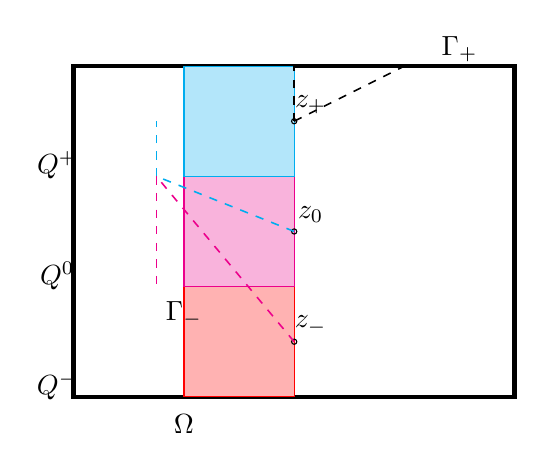
\begin{tikzpicture}[scale=.7]
  \draw[fill=white][ultra thick] (0,0)--(8,0)--(8,6)--(0,6)--cycle;
    \path[draw=red][fill=red!30] (2,0) rectangle (4,2);
     \path[draw=magenta][fill=magenta!30] (2,2) rectangle (4,4);
      \path[draw=cyan][fill=cyan!30] (2,4) rectangle (4,6);
      \node[] at (2,-.5){$\Omega$};
      \node[] at (4,1)[circle,draw=black,scale=.2]{};
      \node[] at (4,3)[circle,draw=black,scale=.2]{};
      \node[] at (4,5)[circle,draw=black,scale=.2]{};
      \node[] at (-.3,.2){$Q^-$};
       \node[] at (-.3,2.2){$Q^0$};
        \node[] at (-.3,4.2){$Q^+$};
         \node[] at (4.3,1.3){$z_{-}$};
          \node[] at (4.3,3.3){$z_{0}$};
           \node[] at (4.3,5.3){$z_{+}$};
            \draw[magenta,dashed][line width=.2mm] (4,1)--(1.5,4);
             \draw[magenta,dashed][line width=.2mm] (1.5,4)--(1.5,2);
              \draw[cyan,dashed][line width=.2mm] (4,3)--(1.5,4);
               \draw[cyan,dashed][line width=.2mm] (1.5,4)--(1.5,5);
                \draw[dashed][line width=.2mm] (4,5)--(6,6);
                 \draw[dashed][line width=.2mm] (4,5)--(4,6);
                  \draw[postaction={decorate},decoration={brace}] (4,6)--(6,6);
                   \node[] at (7,6.3){$\Gamma_{+}$};
                    \node[] at (2,1.5){$\Gamma_{-}$};
                    \end{tikzpicture}